
\documentclass[12pt]{article}
\usepackage[paper=letterpaper,margin=2cm]{geometry}

%\usepackage{coffeestains} %lmao

\usepackage{amsmath}
\usepackage{amsthm} %needed for the proofs 
\usepackage{amssymb}
\usepackage{titling}
\usepackage{thmtools}
\usepackage{mathptmx} %font
\usepackage{verbatim} % for comments
\usepackage{mdframed}
\usepackage[linesnumbered,ruled,vlined]{algorithm2e}
\usepackage{lipsum}

% --- NAMES --- %
\newcommand{\nameone}{Alexandre St-Aubin}
\newcommand{\nametwo}{ and Jonathan Campana}
%images
\usepackage{graphicx}
\graphicspath{ {./images/} }
% to include an image, do: 
%    \begin{center}
%    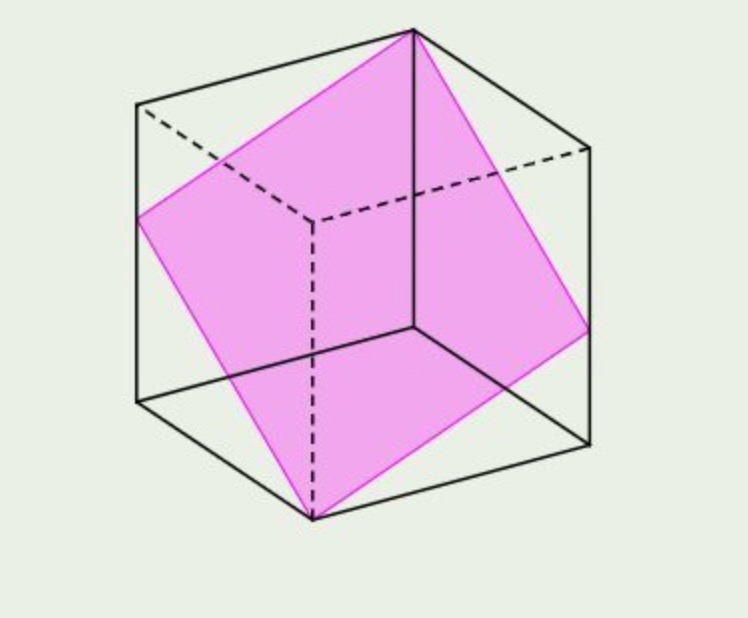
\includegraphics[scale=0.20]{graph.jpg}
%    \end{center}
% OR: 
%\begin{figure}
%    \centering
%    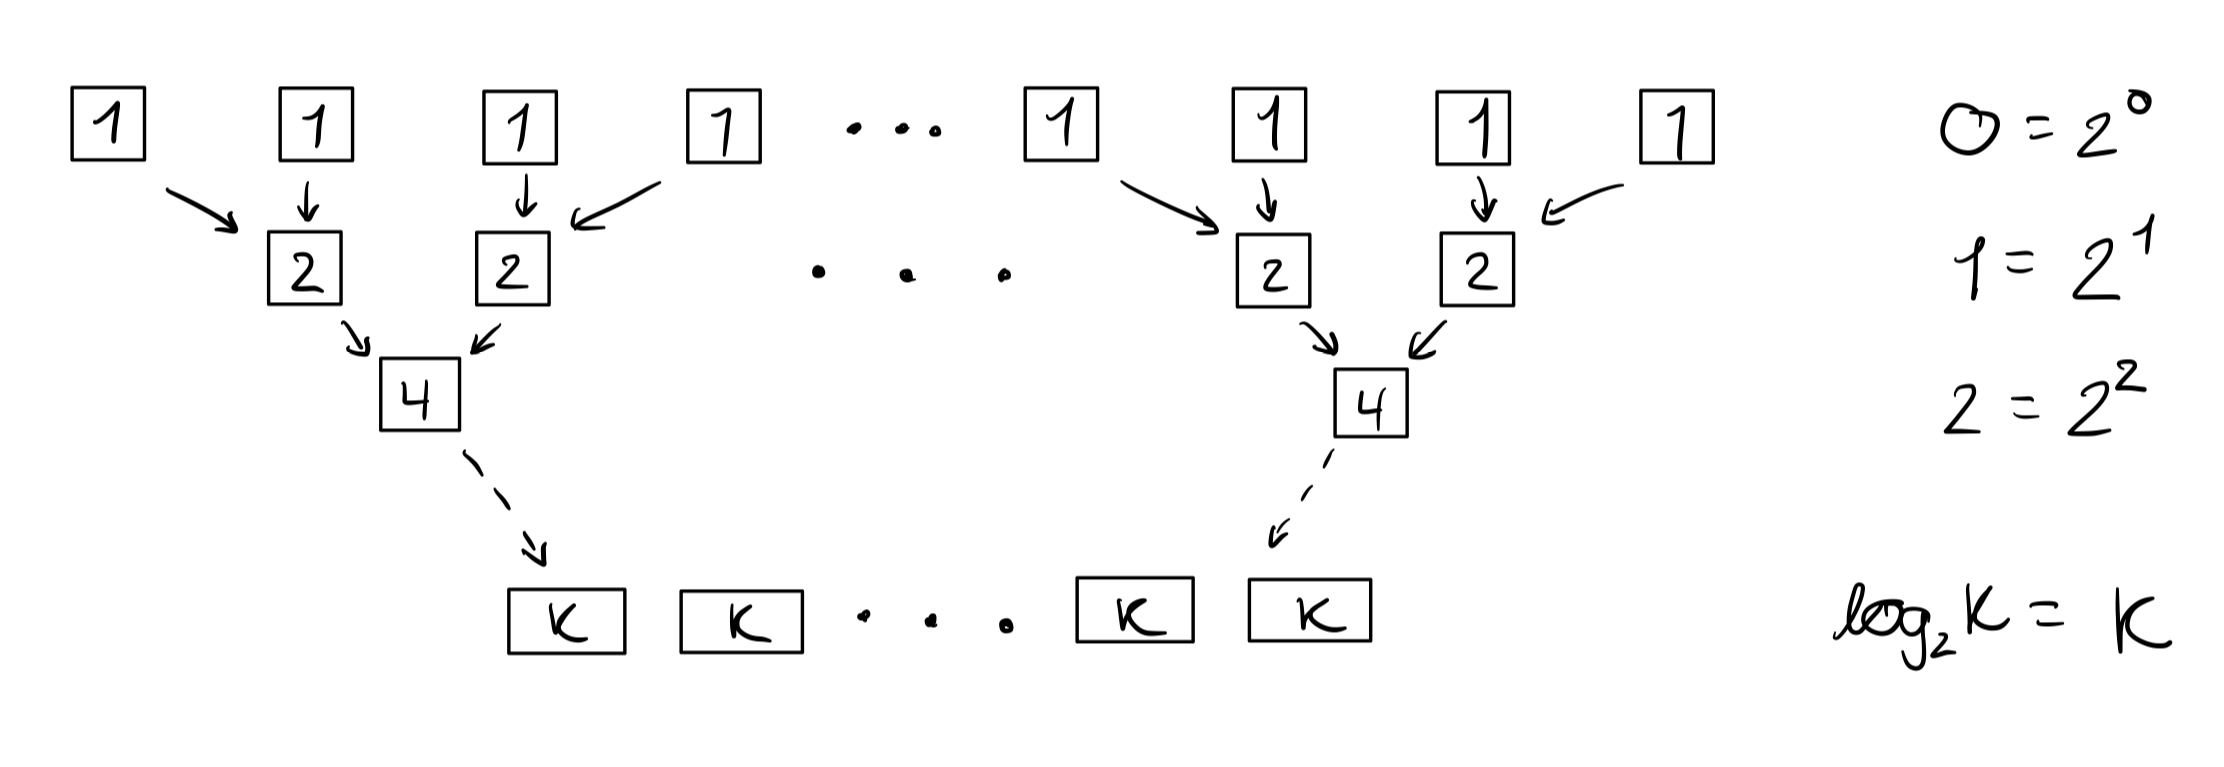
\includegraphics[scale=0.20]{IMG_1052.jpg}
%    \caption{Your caption text here.}
%\end{figure}


%For plots
\usepackage{pgfplots}
\pgfplotsset{compat = newest}

% --- Custom Math Commands --- %
\newtheorem{theorem}{Theorem}
\declaretheoremstyle{lemma}
\declaretheorem[style=lemma, name=Lemma]{lemma}

\theoremstyle{definition}
\newtheorem{definition}{Definition}

\declaretheoremstyle{example}
\declaretheorem[style=example, name=Example]{example}

\theoremstyle{remark}
\newtheorem*{remark}{Remark}

\declaretheoremstyle{proposition}
\declaretheorem[style=proposition, name=Proposition]{proposition}

\declaretheorem[name=Note]{note}
\declaretheoremstyle{note}

\newenvironment{ftheo}
  {\begin{mdframed}\begin{theorem}}
  {\end{theorem}\end{mdframed}}


  % --- Special commands --- %
\newcommand\sol{%
  \\ 
  \\
  \textit{Solution:}\\%
}
% Statistics
\newcommand{\indep}{\perp \!\!\! \perp}
\DeclareMathOperator{\var}{Var}
\DeclareMathOperator{\cov}{Cov}

%Convex optimisation operators
\DeclareMathOperator{\epi}{epi}
\DeclareMathOperator{\lev}{lev}
\DeclareMathOperator{\dom}{dom}
\DeclareMathOperator{\aff}{aff}
\DeclareMathOperator{\ri}{ri}
\DeclareMathOperator{\argmin}{argmin}
\DeclareMathOperator{\conv}{conv}
\DeclareMathOperator{\cl}{cl}


% --- Header --- %
%\renewcommand{\headrulewidth}{.4mm} % header line width

\usepackage[T1]{fontenc} %header
\usepackage[utf8]{inputenc}%header
\usepackage{geometry} %header
\usepackage{fancyhdr}%header
\usepackage{blindtext}
\usepackage{lastpage}

\pagestyle{fancy}
\fancyhf{}
\fancyhfoffset[L]{1cm} % left extra length
\fancyhfoffset[R]{1cm} % right extra length
\rhead{\today}
\lhead{\it \nameone \nametwo}
\fancyfoot[R]{Page \thepage \hspace{1pt} of \pageref{LastPage}}

% --- Title Page --- % 
\setlength{\droptitle}{-6em}

\title{\textsc{Assignment 4 -- COMP 252}}  
\author{\it \nameone \nametwo}
\date{\today}

\begin{document}
\maketitle 
\thispagestyle{empty} %clear first page numbering
%\coffeestainA{0.9}{0.85}{-25}{5cm}{1.3cm}
\begin{enumerate}
  \item \textsc{Browsing the small elements in a red-black tree}. Given is an ordinary red-black tree with a pointer to the smallest element (in addition to a pointer to the root). Cells have five components: left, right, and parent pointers, color of the node, and value of the key.
\begin{enumerate}
  \item We are asked to search for an element u in the tree with key key [u] = x. Show that this can
be done in time $O(1 + \log(k))$ if $x$ is the $k$-th smallest key value stored in the tree (but we only know $x$, not $k$).
\sol
Given a red black tree, we have a balanced binary tree. This means that we can find any element in the RB tree in $\log_2(n)$ time. This also means that we have at most $\lceil \log_2(n)\rceil$ levels to our tree. 

Therefore, starting at the smallest node, we work our way up the RB tree by checking if the key of the node we are at is samller than the node we are looking for (x). We keep doing this until we find a node that has a key that is bigger than the key we are looking for, or we reach a node that does not have a parent nodes (the root). 


Denote the lowest common ancestor as the node that is ancestor to the $k^{th}$ smallest node and the smallest node (our starting point). Given that our nodes are ordered in a red black tree, the possible lowest common ancestors (we will refer to them as LCAs from now on) would be found as the most left nodes of the tree at each level. Denote the possible LCAs
\begin{align*}
    LCA = \{v_1, v_2, \ldots, v_{n}\}
\end{align*}
By the red black tree, we have $\log(n)$ possible LCAs since the tree has n nodes. We, however, will not always reach the root, which is why our complexity is dependent on the $k^{th}$ smallest element rather than $n$. 

By our algorithm, we move to the parent as long as the element we are looking for is bigger than the parent of the node we are currently at. Once we reach the point where the $k^{th}$ smallest element is smaller than the parent node, or the parent node does not exist (the root), we conclude that the element we are searching for must be in the right subtree of the node we are at. 

The $k^{th}$ smallest element in the binary tree can be any element in the right subtree including the current node for the sake of simplicity. Suppose that our LCA is $v_i$. Since the node that contains $k$ is in the right subtree, and the subtree with $v_i$ as the LCA would have at most $2k$ elements inside. 

This is easy to see since the lower bound for the number of leaves in the $v_i$ would be $2k$ (in big Oh) if $key[v_i] = k$, then the left subtree would have $k-1$ elements since that is the number of elements smaller than the node we are looking for, and the right subtree would have at most $k-1$ nodes as well. Suppose that $k$ was farther inside the right subtree, $k$ would be bigger than in the previous case, we could take without loss of generality that the $v_i$ subtree has $2k$ nodes (even though it would have less, since the left subtree wouldn't have k nodes in it) which would give us the same $O(\log(k))$, since the number of levels in this red black $v_i$ subtree is $\lceil \log_2 k \rceil$. 


The second while loop essentially binary searches the right subtree of our LCA $v_i$, which has at most $k$ many nodes in it. Since it takes $O(\log k )$ to binary search a red black tree, this while loop also has $O(\log k)$.

Thus, employing the triangle inequality with this distance metric, we have that 
\begin{align*}
    &d(\text{min pt, } k^{th}) \le d(\text{min pt, greatest common ancestor}) + d(\text{greatest common ancestor, } k^{th}) + 1\\
    &\implies d(\text{min pt, } k^{th}) \le O(\log k + 1) + O(\log k) = O(\log k + 1)\\    
\end{align*}

The constant in our big Oh notation stems from the possibility that $k=1$, where $\log k = 0$, but there is still a comparison, so we add the 1. 

  \item[\it (ii)] Give the algorithm for part (i).

\begin{algorithm} 
    \caption{Find\_kth\_smallest red-black tree.}
    \SetKwProg{Fn}{Function }{\string:}{}
    \SetKwRepeat{Do}{do}{while} %do-while loop macro
    \SetKwInput{KwOut}{Output}
    \SetKwInput{KwIn}{Input}
    \SetKwFunction{rad}{Radius}
    \SetKwFunction{cen}{centre\_dist}
    \SetKwData{dec}{possible\_adjacent\_stack}
    \SetKwData{a}{a}
    \SetKwData{b}{b}
    \SetKwData{np}{node\_pointer}    
    \SetKwData{ltok}{left\_to\_circle}   
    \SetKwData{maxd}{max\_d}   
    \SetKwData{null}{NULL}  
    \SetKwData{wid}{Width}   
    \SetKwFunction{mn}{MAKENULL}
    \SetKwFunction{top}{PEEK}
    \SetKwFunction{pop}{POP}
    \SetKwFunction{push}{PUSH}

    \KwIn{Pointers to the smallest element and root of a red black tree, and value of $x$. }
    \KwOut{Finds node of value $x$ in the tree.}
    \BlankLine
    \While{$(x \geq \text{key}[\np])$}{
        \If{$\text{key}[\np] = x$}{
             \Return $\np$;
        }
        \eIf{$(\text{key}[\text{parent}[\np]] \neq \null)$}{
            $\np \gets \text{parent}[\np]$;
        }{
        \textbf{break};
        }
   }    
    $\np \gets \text{right}[\text{left}[\np]]$ \tcp{\color{blue}The parent was bigger than $x$, thus we go back in the subtree and set our pointer to the right child}
    
    \While{$(x \neq \text{key}[\np]) \land (\text{key}[\np] \neq \null)$}{
        \eIf{$x > \text{key}[\np]$}{
            $\np \gets \text{right}[\np];$
        }{
        $\np \gets \text{left}[\np];$
        }
    }
    
    \eIf{$x = \text{key}[\np]$}{
      \Return $\np$;
    }{
       \Return \null;
    }
    
\end{algorithm}
\end{enumerate}
  \newpage 
  \item \textsc{Greedy algorithm}. On a flat table, we have placed n disks of radii $r_1, ..., r_n$, numbered from left to right. We push them together without creating overlap, as in the figure below. Give an $O(n)$ time algorithm to compute the size of the smallest axis-aligned rectangle that can hold the disks.
  \sol 
  See the algorithm on the next page. We show that its complexity is $O(n)$. To begin, the outermost loop at line 8 iterates a total of $n$ times. The maximum number of elements pushed onto the stack is also $n$ (since at most one is pushed at each iteration), hence an equal number is removed, maintaining the overall $O(n)$ complexity. Finally, as we traverse through each circle once more at the end of the algorithm, the complexity remains $O(n)$.
  \begin{algorithm}
    \caption{Greedy circle packing}
    \SetKwProg{Fn}{Function }{\string:}{}
    \SetKwRepeat{Do}{do}{while} %do-while loop macro
    \SetKwInput{KwOut}{Output}
    \SetKwInput{KwIn}{Input}
    \SetKwFunction{rad}{Radius}
    \SetKwFunction{cen}{centre\_dist}
    \SetKwData{dec}{possible\_adjacent\_stack}
    \SetKwData{a}{a}
    \SetKwData{b}{b}
    \SetKwData{arr}{array}    
    \SetKwData{ltok}{left\_to\_circle}   
    \SetKwData{maxd}{max\_d}   
    \SetKwData{len}{length}  
    \SetKwData{wid}{Width}   
    \SetKwFunction{mn}{MAKENULL}
    \SetKwFunction{top}{PEEK}
    \SetKwFunction{pop}{POP}
    \SetKwFunction{push}{PUSH}

    \KwIn{An ordered list $\Omega := \{1,2,3,...,n\}$ of $n$ circles. }
    \KwOut{The minimum width of a rectangle that can hold the disks.}
    \BlankLine

    \tcp{\color{blue}radius of the circle a}
    \Fn{\rad{circle \a}}{
        \Return radius of \a;
    }
    \BlankLine

    \tcp{\color{blue}distance between the centres of a and b if they are pushed together.}
    \Fn{\cen{circle \a, circle \b}}{
      \Return $ \sqrt{(\rad(a)+\rad(b))^2 -(\rad(a)-\rad(b))^2};$
    }
    \BlankLine 
    \tcp{\color{blue}largest subarray of $\Omega$ ending with $k$, decreasing in radii. }
    $\mn (\dec); $\\
    \BlankLine 
    \tcp{\color{blue}distance from the left side of the rectangle to circle at index}
    $\ltok[] \gets new \; \arr;$\\     
    \BlankLine
    $\ltok[0] \gets 0;$\\ 

    \For{all $i \in \Omega$}{
      \eIf{$i=1$}{
        $\ltok[i-1] \gets \rad(i);$\\
        $\push(i, \dec)$\\ 
      }{
        \tcp{\color{blue} initialize \maxd, the maximum distance between left side of rectangle and circle i to \rad(i). to account for the case where the circle would touch the side of the rectangle.}
        $\maxd \gets \rad(i);$\\
        \tcp{\color{blue} \pop each circle on the stack that's smaller than i.}
      \While{$\rad(\top{\dec}) \leq \rad(i)$}{
        $\maxd \gets \max\{\maxd, \ltok(\pop{\dec})+ \cen(i, \dec(j)) \} ;$
      }
      \tcp{\color{blue} peek the first circle that's larger, but keep it on the stack}
      $\maxd \gets \max\{\maxd, \ltok(\top{\dec})+ \cen(i, \dec(j)) \} ;$\\ 
      \tcp{\color{blue}push i to stack, keeping the decreasing order}
      $\push(i, \dec);$\\ 
        \tcp{\color{blue} \maxd is the distance from the left side of the rectangle to the center of circle i when it is pushed as much as possible without overlapping}
        $\ltok[i-1] \gets \maxd;$\\ 
      }
      }
    \tcp{ \color{blue} find the width}
    $\wid \gets 0;$\\ 
    \For {$i \gets n-1 \text{ to } 0$}{
      \If{$\ltok[i]+ \rad(i)>\wid$}{
          $\wid \gets\ltok[i]+ \rad(i);$\\ 
      }
    }\Return \wid;
    
  \end{algorithm}
 \newpage 
  \item \textsc{Augmented data structures.} Show how to maintain a dynamic set of numbers that
supports the operation \texttt{min-gap}, which gives the magnitude of the difference of the two closest numbers in a set of numbers, A. For example, if $A = \{1, 5, 9, 15, 18, 22\}$, then \texttt{min-gap} $(A)$ returns $18 - 15 = 3$, since 15 and 18 are the two closest numbers in $A$. Make the operations \texttt{insert, delete, search}, and \texttt{min-gap} as efficient as possible, and analyze the running times. Be concise! 
\newpage 
\item \textsc{The node of smallest tension in a tree.} Given is an unrooted free tree of size $n$.
The nodes are labeled from $1$ to $n$, and for each node, we have a linked list of its neighbors. When a node $u$ is deleted, it breaks the tree up into a forest of disjoint trees, say $T_1, ... , T_k$. Let the sizes of these trees be denoted by $|T_1|,... , |T_k|$. We define the tension of $u$ as $\max_{1 \leq i \leq k} T_i$. The objective is to find a node $u$ of smallest tension. Intuitively, it should be near the “center” of the tree. Write an algorithm
that takes $O(n)$ worst-case time.
\sol 
See the algorithm on the next page. The complexity is easily seen to be $O(n)$, given that line 21 executes at most $n$ times, and both loops at lines 28 and 34 iterate $n$ times. Additionally, the post\_order\_traversal function is $O(n)$, as it traverses every node in the tree. 

The algorithm uses the following data structure, 
\begin{equation*}
  \begin{split}
    &\texttt{struct NODE}\\ 
    &\{\\ 
    &\texttt{linkedList } \text{neighbour}; \\ 
    &\texttt{int } \text{tension}; \\ 
    &\texttt{int } \text{size} ;\\ 
    &\texttt{bool }\text{visited}; \\
    &\}\\
  \end{split}
\end{equation*}

\begin{algorithm}
    \caption{Smallest Tension}
    \SetKwProg{Fn}{Function }{\string:}{}
    \SetKwInput{KwOut}{Output}
    \SetKwInput{KwIn}{Input}
    \SetKwFunction{stru}{struct}
    \SetKwData{true}{True}
    \SetKwData{chi}{child}
    \SetKwData{parent}{parent}
    \SetKwData{ten}{tension}
    \SetKwData{size}{size}
    \SetKwData{visited}{visited}    
    \SetKwData{root}{root}
    \SetKwData{toproot}{TopRoot}
    \SetKwData{nei}{neighbours}   
    \SetKwData{false}{False}  
    \SetKwData{null}{NULL}   
    \SetKwFunction{mn}{MAKENULL}
    \SetKwFunction{top}{PEEK}
    \SetKwFunction{pop}{POP}
    \SetKwFunction{isemp}{ISEMPTY}
    \SetKwFunction{potrav}{post\_order\_traversal}
    \SetKwFunction{exit}{exit}
    \SetKwFunction{init}{initialize}
    \SetKwData{temp}{temp}
    \SetKwData{continue}{continue}

    \KwIn{A list $\Omega := \{1,2,3,...,n\}$ of nodes, and for each node, a linked list of neighbours.}
    \KwOut{The node of minimum tension.}
\BlankLine
\Fn{\potrav{\root}}{
    $\root.\visited \gets \true;$\\
    \If{$|\root.\nei| = 1$}{
        $\root.\size \gets 1; $\\ 
        $\root.\ten \gets n-1;$\\
        \Return ;
    }
    \ForAll{ \texttt{NODE} $\chi$ in $\root.\nei$}{
        \If{$\chi.\visited = \true$}{\continue\tcp{\color{blue} means the node is a parent, so don't visit.}}
        \potrav{$\chi$};
    }
    \tcp{\color{blue}visit node}
    
    \ForAll{ \texttt{NODE} $\chi$ in $\root.\nei$}{
        $\root.\size \gets \root.\size + \chi.\size$; \tcp{\color{blue}one of the nodes is going to be the parent, but since it hasn't been visited yet, its field \texttt{size} will be 0, so this is an accurate calculation of the size.}
    }
    $\root.\ten \gets \max \{\max_{i \in \root.\nei} \{i.\size\}, n - \root.\size\} $;\\ 
    \Return; 
  } \tcp{\color{red}--- Driver code ---}
 \tcp{\color{blue} add fields to each node.}
       \ForAll{$i \in \Omega$}{      
       $\temp \gets i.\nei;$\\ 
      $i \gets new \texttt{ struct } \texttt{NODE}$;\\  
      $i.\visited \gets \false;$\\ 
      $i.\nei \gets \temp ;$\\ 
      $i.\ten \gets 0;$\\ 
      $i.\size \gets 0;$
    }
    \tcp{\color{blue} find a node that's not a leaf and initialize it as root.}
    \ForAll{$i \in \Omega $}{
      \If{$|i.\nei| >1$}{
      $\toproot \gets i;$\\ 
      \exit;
      }
    }
    \tcp{\color{blue} call the traversal at the top root}
    $\potrav(\toproot)$;\\
    $\temp \gets \infty ;$\\ 
    \For{all $i\in \Omega$}{
      \If{$i.\ten < \temp$}{
        $\temp \gets i.\ten$;
      }
    }
    \Return $\temp;$
    \end{algorithm}

\end{enumerate}
\end{document}
